% XeLaTeX
%\documentclass[tikz, border=5mm, convert, convert={outext=.svg, command=\unexpanded{
%    pdf2svg \infile\space \outfile\space all
%    }}]{standalone}
\documentclass[tikz, border=5mm, convert={outext=.png}]{standalone}
\usepackage{fontspec}
\setmainfont{Avenir}

\begin{document}
    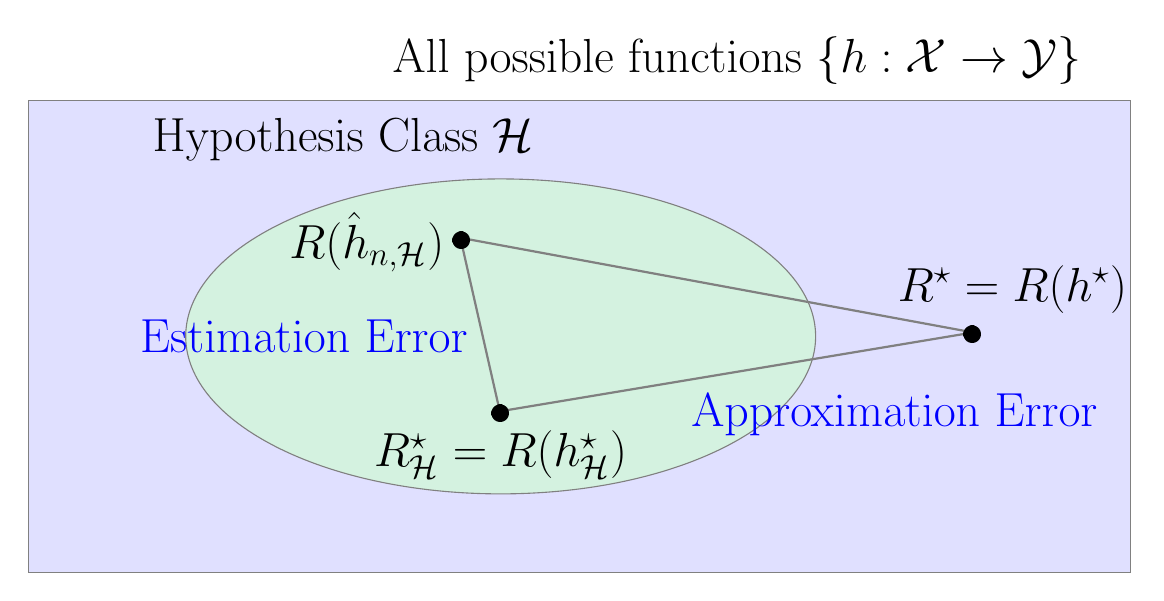
\begin{tikzpicture}
        \begin{scope} [fill opacity = .6]
            \draw[fill=blue!20, draw = gray] (-7,3) rectangle (7,-3);
            \draw[fill=green!20, draw = gray] (-1,0) ellipse (4cm and 2cm);
        \end{scope}
        \node at (2,3.5) {\LARGE All possible functions $\{h:\mathcal{X} \to \mathcal{Y}\}$};

        \draw[gray, thick] (5,0.05) -- (-1,-0.95);
        \draw[gray, thick] (-1.5, 1.2) -- (-1,-1);
        \draw[gray, thick] (5,0.05) -- (-1.5,1.25);

        \node at (-3,2.5) {\LARGE Hypothesis Class $\mathcal{H}$};
        \node at (5,0) {\LARGE \textbullet};
        \node at (5.5,0.6) {\LARGE $R^{\star} = R(h^{\star})$};
        \node at (-1,-1) {\LARGE \textbullet};
        \node at (-1,-1.5) {\LARGE $R^{\star}_{\mathcal{H}} = R(h^{\star}_{\mathcal{H}})$};
        \node at (-1.5,1.2) {\LARGE \textbullet};
        \node at (-2.7,1.2) {\LARGE $R(\hat{h}_{n,\mathcal{H}})$};

        \node at (-3.5,0) {\LARGE \textcolor{blue}{Estimation Error}};
        \node at (4,-1) {\LARGE \textcolor{blue}{Approximation Error}};

    \end{tikzpicture}
\end{document}